\documentclass[a4paper,pagenum,english]{rnti}
\usepackage{graphicx}
\usepackage{listings}

\usepackage[T1]{fontenc}
\usepackage[latin1]{inputenc}
\usepackage{url}


\usepackage{xcolor}

\colorlet{punct}{red!60!black}
\definecolor{background}{HTML}{EEEEEE}
\definecolor{delim}{RGB}{20,105,176}
\colorlet{numb}{magenta!60!black}

\lstdefinelanguage{json}{
    basicstyle=\normalfont\ttfamily,
    numbers=left,
    numberstyle=\scriptsize,
    stepnumber=1,
    numbersep=8pt,
    showstringspaces=false,
    breaklines=true,
    frame=lines,
    backgroundcolor=\color{background},
    literate=
     *{0}{{{\color{numb}0}}}{1}
      {1}{{{\color{numb}1}}}{1}
      {2}{{{\color{numb}2}}}{1}
      {3}{{{\color{numb}3}}}{1}
      {4}{{{\color{numb}4}}}{1}
      {5}{{{\color{numb}5}}}{1}
      {6}{{{\color{numb}6}}}{1}
      {7}{{{\color{numb}7}}}{1}
      {8}{{{\color{numb}8}}}{1}
      {9}{{{\color{numb}9}}}{1}
      {:}{{{\color{punct}{:}}}}{1}
      {,}{{{\color{punct}{,}}}}{1}
      {\{}{{{\color{delim}{\{}}}}{1}
      {\}}{{{\color{delim}{\}}}}}{1}
      {[}{{{\color{delim}{[}}}}{1}
      {]}{{{\color{delim}{]}}}}{1},
}


\titrecourt{GeoCarteApp: A generic and personalized tool for the visualization of geospatial data}

\nomcourt{I. Bakerally et al.}


\titre{GeoCarteApp: A generic and personalized tool for the visualization of geospatial data}

\auteur{Noorani Bakerally\affil{1},
        Ghislain Atemezing\affil{2}\\
        Antoine Zimmermann\affil{1},
        Olivier Boissier\affil{1}}

\affiliation{
    \affil{1}Univ Lyon, MINES Saint-\'Etienne, CNRS, Laboratoire Hubert Curien UMR 5516, \\F-42023 Saint-\'Etienne, France\\
          \{prenom.nom\}@emse.fr\\
    %
    \affil{2}Mondeca, \\ 35 boulevard Strasbourg, Paris, France\\
          ghislain.atemezing@mondeca.com\\
          %\http{http://www.mondeca.com}
 }




\summary{GeoSpatial data is becoming more and more important in numerous domains. Many standards related to geospatial data such as GeoSPARQL or GML have been defined to facilitate interchange, reasoning and querying of geospatial data on the Web. However, there are still many datasets provided by organizations and open data portals which provide unstructured geospatial data. However, there is a need for such a tool which can help domain experts to bring different types of geospatial data, whether standardized, partially standard or heterogeneous data on a single map for analysis. In this paper, we provide a tool, GeoCarteApp, which can allow the visualization of geospatial data irrespective of the data model or format through the use of default or personalized configurations. We describe the tool, its features and show its usefulness for the trees' dataset related to Grenoble}

\begin{document}
\section{Introduction}
Currently, much data is available from open data portals. These data are encoded in different formats and based on different data models. Much of these data are geospatial data about different themes such as transportation, public services or tourism. These data are based on different data models, sometimes proprietary or sometimes standard. Due to the heterogeneity of geospatial data, map APIs (like Google Maps or MapBox) cannot directly consume the data for visualization purposes. As of now, map applications may directly consume data in GeoJSON, KML, ShapeFile and some others directly. For example, using Google Maps, one may drag and drop a GeoJSON data or text on a map and directly visualize the data. However, this is not yet directly possible for data in different formats and model like RDF, CSV, JSON etc. For example, the LinkedGeoData~\cite{stadler2012linkedgeodata} is a rich source of geospatial data which provides information collected by OpenStreetMap project and makes it available as RDF via their SPARQL endpoint \footnote{\url{http://linkedgeodata.org/sparql}} and RDF datasets. SPARQL queries can be written to obtain useful information from this source however the SPARQL results cannot be directly consume by map APIs for visualization. Same is the case for GeoNames or DBpedia and other rich sources of geospatial data. To allow the map application to consume data from heterogeneous sources, one has to programmatically parse the file and use the API to visualize the data on a map which can be a limitation for organization or domain experts not possessing the technical skills to do so.

This problem can be solved by using a generic approach which can allow data of different data models and formats to be automatically visualized on a map. In this paper, (1) we provide a description of the generic approach to generate a default visualization of geospatial data on a map in Section \ref{section:generic}, (2) we explain how this default visualization can be customized through configuration files to allow users to personalize the visualization according to their own preferences in Section \ref{section:customisation}, (3) we consider how this generic approach can help in case of Grenoble ....




To demonstrate this approach, we provide the description of a generic approach.....


\section{GeoCarteApp: A Generic Approach}\label{section:generic}
\begin{figure}
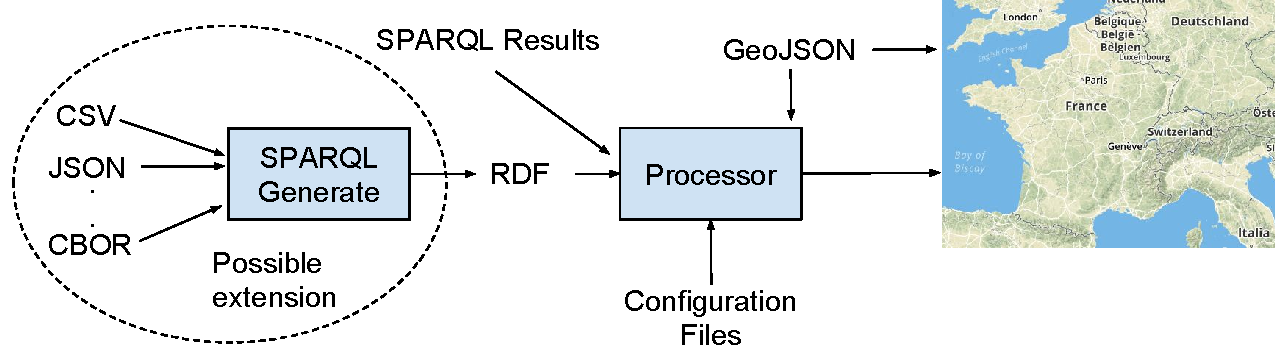
\includegraphics[scale=0.6]{img/generic_approach.pdf}
\caption{Generic Approach to visualize RDF Spatial data}
\label{fig:generic}
\end{figure}

\begin{figure}
\center
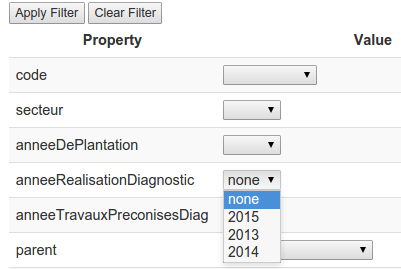
\includegraphics[scale=0.5]{img/default_filter.png}
\caption{Default filters for trees}
\label{fig:default_filter}
\end{figure}

\begin{figure}
\center
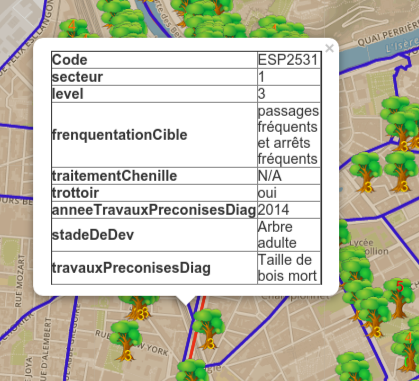
\includegraphics[scale=0.5]{img/default_description.png}
\caption{Default description for a sector in Grenoble}
\label{fig:default_description}
\end{figure}

In this section bla bla bla.... layers, data sources, filtering mechanism, default description..

types of layers in map:
	- marker
	- vector
forms part of a similar layer group	
By data source, we refer to ..,..,..

\subsection{Instantiation of the Generic Approach}
- brief description of an application which uses this generic approach.....
- two different configurations..

\subsection{Description of the Generic Approach}
Figure \ref{fig:generic} provides a high-level architecture of GeoCarteApp. As it be seen, the generic processor can consume RDF, SPARQL results and GeoJSON. As of now, the processor cannot consume data in other heterogeneous formats. But it can be easily further enhanced by using SPARQL Generate  \footnote{http://ci.emse.fr/sparql-generate/} which produces RDF equivalents of data in formats like CSV, JSON, CBOR and others. These RDF equivalents can then be directly input to the generic processor. 



The generic processor can consume geospatial data from RDF, SPARQL result and GeoJSON to produce a default visualization. 


As of now, the processor can only consume RDF. But it can be easily further enhanced by using SPARQL Generate \footnote{\url{http://ci.emse.fr/sparql-generate/}} which produces RDF equivalents of data in other formats. These RDF equivalents can then be used as input to the generic processor.


The default visualization of RDF data is possible only due to standards like GeoSPARQL~[\cite{perry2012ogc}] and Linked Data best practices, like using the WGS84 vocabulary which is highly used by many datasets for encoding geographic coordinates~[\cite{schmachtenberg2014adoption}]. However, if these vocabularies are not used, it is still possible to visualize the data by using customized configurations.

The generic processor can also consume SPARQL results. In this case, the generic processor will require at least 3 items of data. Firstly,  the variable corresponding to the latitude and longitude in the SPARQL result must be specified. Then, both the URL for the SPARQL endpoint and the SPARQL query must be provided. The SPARQL endpoint is then queried with the query and the SPARQL results are processed. For each solution, the processor creates a layer.

GeoJSON can be directly consume by map APIs like Google Maps\footnote{\url{https://developers.google.com/maps/}} or MapBox\footnote{\url{https://www.mapbox.com}}. However, when consumed via the generic processor, default unique colors are applied to the rendered GeoJSON layers to ensure that it is distinguished among other map layers. This is particulary important if one is making a map mashup whereby data from numerous sources are bring on a single map.

Besides rendering layers on the map, the generic processor does two more things. While processing the data sources, it collects the properties and property values for the objects to be shown on the map. If source is an RDF source, all the property and their values are collected for each unique object. If SPARQL result is used, all variable and their bindings are collected. Finally, if the source GeoJSON, for each object in the \texttt{features} list, the properties and their values are collected from the \texttt{properties} object. Using all these properties and their values for a particular object, the generic processor generates a set of properties and a set of possible values for each properties. Using this, the application provides a default filtering mechanism which can be used to search for specific objects on the map.

Figure \ref{fig:default_filter} shows part of the user interface for default filters of Grenoble trees which comes from a SPARQL result. Similar default filters will be generated if the data source is RDF or GeoJSON. As shown in that figure, there is a set of properties and a set of property values for each property. By default, the selected value for each property is \texttt{none}. After choosing the appropriate value for each property, when filters can be applied. A property having whose value is \texttt{none} will be ignored in the filters. After applying the filters for a particular layer group, only those objects will be shown on the map which satisfy all the filters. As of now, an object is shown only if its properties and property values satisfy all the filters, i.e. the filter expression is a logical AND of all the filters. This semantic can be further enhanced in future versions of the application where filter expression may be a logical OR or XOR of all filters.


A sample of this default visualization can be seen in Figure... 


The generic processor can generate a default description for each object. The map API then binds this default description to that object. When the object is shown on the map, on clicking on it, the description is shown in a popup as shown in Figure \ref{fig:default_description}
\begin{lstlisting}[language=json,firstnumber=1, caption={Sample default configuration file}\label{listing:default_configuration}]
{"FranceGeoNames": {
	"dataSource": {
	"type": "RDFDataSource",
	"url": "http://www.geonames.org/3017382/about.rdf"
	}
},"Ecoles élementaires": {
	"dataSource": {
	"type": "GeoJSONDataSource",
	"url": "http://sig.grenoble.fr/opendata/Decoupage/json/DECOUPAGE_%C3%89L%C3%89MENTAIRES_EPSG4326.json"
	}
},"Arbres": {
	"latCol": "lat",
	"longCol": "long",
	"dataSource": {
	"type": "SPARQLDataSource",
	"url": "http://data.mondeca.com/egc2017/sparql",
	"query": "The SPARQL Query goes here"
}
}}
\end{lstlisting}
As shown in Listing \ref{listing:default_configuration}, to produce the default visualization, for RDF, the processor only needs the URL of the RDF file. It then follows GeoSPARQL and WGS84 vocabulary to extract the geospatial data. The processor can also consume SPARQL results. For the set of solutions from the SPARQL results, the column for the latitude and longitude should be specified. Like RDF, a GeoJSON file can stating its URL.

\section{Customisation/Configuration (source)}\label{section:customisation}
GeoCarteApp can provides a default visualization with default colors, filters and layer descriptions. However, users may want to customize the configurations to obtain a personalize visualization. The customizations of the configurations can be categorized mainly in four categories. They are:
\begin{enumerate}
\item Layer
\item Filter
\item Rendering
\item Datasource
\end{enumerate}

\subsection{Datasource Customizations}
If the datasource is SPARQL result, by default, the generic processor considers each solution as a separate object and from which it generates a unique layer. However, it is possible that a SPARQL Results contains two different solutions which corresponds to a single object. For example, this can arise if a single subject occurs in at least two different triples with the same predicates but different objects. If the default configuration is used, the generic processor will create a distinct objects for each solution. To prevent this issue, a further property \texttt{identifier} can be added to the \texttt{datasource} description to tell the processor which variable binding to consider as the identifier. Finally, using the identifier, when the generic processor process the solutions, it creates a single object for solutions having similar identifier. 

Moreover, when the datasource is RDF, by the default, the generic processor considers all subjects having a latitude and longitude description following the WGS84 vocabulary~[\cite{brickley2003w3c}]. However, it is possible that the RDF vocabulary uses a different vocabulary. To ensure that the generic processor finds the latitude and longitude description, two additional properties \texttt{latitudeProperty} and \texttt{longitudeProperty} can be added to the \texttt{datasource} to specify the property used for latitude and longitude respectively.

Moreover, when the generic processor process the RDF file, it considers all subjects having a latitude and longitude description. The set of subjects to be considered can be limited by one or more classes by adding a property \texttt{class} to \texttt{datasource}. The value for this property can be a string to denote one class or a list consisting more than one class. If there is more than one class, a subject is chosen if it is an instance of any one of the classes.

\subsection{Visualization Customizations}
By default, the generic processor generates a default description for each object in a layer group. It is possible to configure it so that there is no description or a custom description. The custom description will take the form of a string marked up with a property. For example, suppose an object has three properties namely code, latitude and longitude with values 234, 45 and 5 respectively. A custom description can be of the form "The sector \{code\} has latitude \{latitude\} and longitude \{longitude\}". The processor will then replace the property value for the three properties can generate a description like "The sector 234 has latitude 45 and longitude 5". Then, if a string has to contain the special character \{ or \}, it will have to escaped. 

Also, it is possible to generate derived properties for objects. For example, in the case of Grenoble data, it is known that a particular tree was planed in a particular year. It is possible to have a new property "age" and calculate the age of the tree. Different icons and colors can be specified for both marker and vector layer groups. Further, marker and vector layers can have different appearences like color, border color, inside color or icon based on the properties of their respective objects. For example, trees in different age intervals can have different icons.

It may happen that a particular layer groups have thousands of objects. Due to resource limitations, it may not be possible to show all the objects from that layer group on the map. In this case, topological relationships namely contains can be used to limit the number of layers being rendered. In the Defi 2 for EGC 2017, there are 10251 trees. On our web application, displaying all the trees was taking much time and even when displayed, the application was lagging. In short, the the \texttt{areaConstraint} creates a dependency between two layers. The Figure \ref{fig:default_filter} TO CHANGE shows an example of the application of the \texttt{contains} constraint. In this case, there are three layers involved which corresponds to Grenoble Sectors, subsectors and trees. The sectors and subsectors act as an \texttt{containts} constraints for trees, which means that a particular must be simultenenously in a particular sector and subsector to it to be shown on the map. As a result, by using filters, a particular sector and subsector can be shown and only trees within this sector and subsectors can be rendered.

\subsection{Filter Customizations}
As shown in Figure \ref{fig:default_filter}, there is a label for each property and for each value. These labels are taken raw as they are from the datasource. As it can be seen both in Figure \ref{fig:default_filter} and \ref{fig:default_description}, the labels for the property and values follows some database or arbitrary conventions. Configurations can be used to allow for more user-friendly labels both for property and property values. Furthermore, by default, all properties and all values for a particular property are considered in the Filters' section of the user interface. In the configuration, it can be explicitly stated which property or property values to include or exclude.

\section{Application to Grenoble Data}\label{section:customisation}
We apply our generic approach to visualize geospatial data in the domain of environment, in particular to monitor trees in the city of Grenoble. To that purpose, we first convert the legacy datasets into the RDF model, based on a vocabulary. Then we enrich the dataset with relevant datasets according to our use cases, and then we show how our application can be used by domain experts.

\subsection{Transformation and Enrichment of Data}

\subsection{Transformation}
% ontologies used and RDF conversion
The model use for the conversion of the CSV data is based on 2 classes, 4 object properties and 25 datatypes\footnote{\url{https://goo.gl/FTFGbh}}.  
We use the lgdo:Tree\footnote{\url{http://linkedgeodata.org/ontology/}} to represent the main class. The class \textit{tonto:Sector} is a sublass of a topological entity \textit{topo:EntiteTopographique}\footnote{\url{http://data.ign.fr/def/topo#}}. 


\subsection{Enrichissement}
% Add here the work done to enrich original dataset

	- We added information about allergy-inducing trees from Wikipedia: %https://fr.wikipedia.org/wiki/Liste_des_plantes_allergisantes
We used dataset from 
%https://fr.wikipedia.org/wiki/Liste_des_plantes_allergisantes
 and converted it in RDF to enrich the original dataset with information on allergy for the species of the trees found in Grenoble. 
 
linkedgeodata



% We added information about allergy-inducing trees from Wikipedia: https://fr.wikipedia.org/wiki/Liste_des_plantes_allergisantes
%We used dataset from https://fr.wikipedia.org/wiki/Liste_des_plantes_allergisantes and converted it in RDF to enrich the original dataset with information on allergy for the species of the trees found in Grenoble. 


\section{Use Cases}
- search for trees which have to be diagnose
- specific icon for trees with allergies
- others: See Q8 for more info from DBpedia regarding species if needed to enrich more our dataset.
- Species which can create allergies
- schools + hospital + allergy
- post offices in Grenoble  see query 7 here %https://github.com/gatemezing/egc2017/blob/master/queries/example-queries.sparql 
- Species from DBPedia
- Species from DBPedia (see Q8 for a sample query)
- frequentation cible + allergy
\section{Recommendation on the Data}
% in French, to be translated
Les donn�es de localisation propos�es dans ce d�fi souffrent du manque des m�tadonn�es n�cessaires pour faciliter leur exploitation, au moins sur deux aspects importants: le type de coordonn�es g�ographiques et la correspondance des (X,Y) par rapport aux latitudes et longitudes. Ces �l�ments sont fondamentaux pour faciliter la r�utilisation des donn�es g�ographiques, surtout en qui concerne le positionnement et la meilleure interpr�tation des objets contenus dans les donn�es. Il a fallu d�terminer par des scripts ad hoc que les donn�es g�ographiques utilisaient du EPSG:3945 (RGF 93/CC45) en limitant aux syst�mes de coordonn�es utilis�es en France. 
De m�me, entre les diff�rents fichiers il n?existe pas de relation ?explicite? permettant de les relier entre elles, comme les cl�s dans les bases de donn�es. Ce manque d?information n�cessite un travail suppl�mentaire pour l?utilisateur des donn�es de faire une inf�rence bas�e sur le m�me nombre de lignes dans les diff�rents fichiers pour faire une corr�lation de similarit� bas�e sur les lignes.
Nous pr�conisons de mettre explicitation sur les m�tadonn�es des informations de syst�mes de coordonn�es, ainsi que la mention de relations existantes entre les diff�rents fichiers � exploiter par les utilisateurs. 

\section{Conclusion and Perspectives}
More and more geospatial data is now available with the idea of open data. This can create interesting usage use cases for both normal citizens and organizations. Map mashups can be created and provided on the Web for day to day scenarios or for analysis by domain experts. However, there is a lack of tool for the on-the-fly consumption of geospatial data in any format for visualization purposes. To our knowledge, there is no proposed approach for directly consuming geospatial data for map visualization from any data format. To this end, we propose a generic approach which can work without any configurations. We also propose the ability to define customisations in a configuration file to produce highly personalized visualization and filtering. As a proof of concept, we provide a toy application on the Web which is though not optimized but is fully function. As of now, using the application may be complex for non-technical users. This is because configuration files needs to be hand written. As a perspective, we consider the possibility of having user interfaces to help non-technical users in automatically generating configurations. Moreover, the configurations is not yet fully finalized and it will be an opportunity to have a vocabulary for to concertize the configurations and enhance its usage by interested parties. Last but not least, our future work includes the extension of this approach to consider other data formats such CSV, JSON and others. 
\paragraph{Acknowledgements} This work has been done within the OpenSensingCity project, supported by ANR (Agence Nationale de la Recherche), Project ID: ANR-14-CE24-0029.

\bibliographystyle{rnti}
\bibliography{biblioaz}
\end{document}
